\chapter{The LHCb Detector}

The data used in this thesis originates from the LHCb Detector at the particle collider LHC or simulations thereof.
This detector is mainly focused on decays in which a bottom or a charm quark is involved to do precision measurements on the CP-violation and on rare decays. 
To accomplish this it has been build as a single arm forward-spectrometer, because the majority of $b$-/$c$-Hadron pairs are produced with velocities inside a cone around the beampipe.
An overview of the detector is shown in \autoref{fig:lhcb_detector}.
Its components are described briefly in this chapter.

\begin{figure}
    \centering
    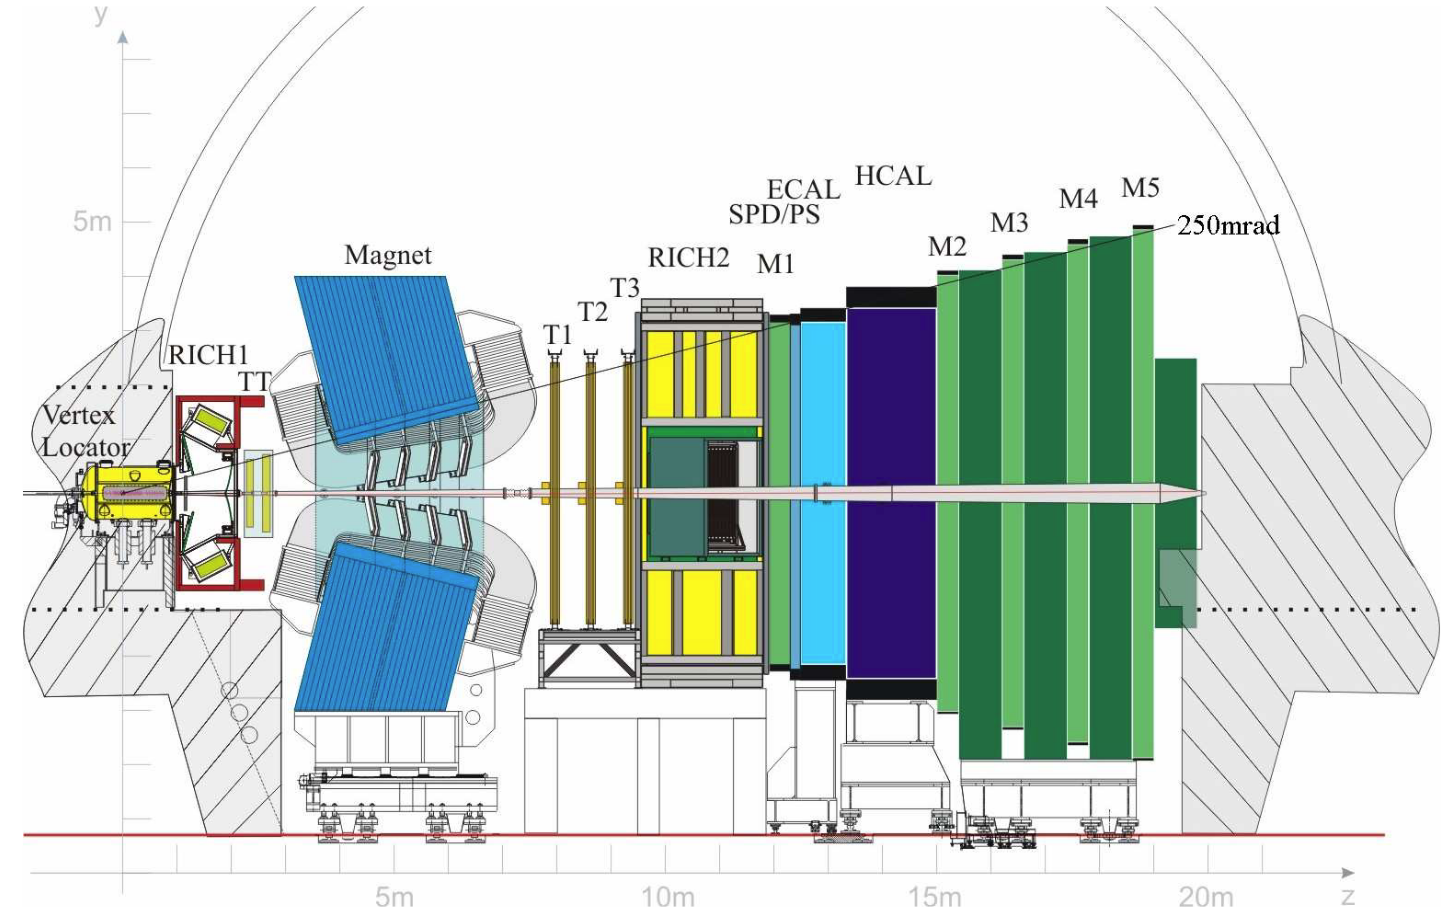
\includegraphics[width=\textwidth]{images/lhcb_detector.png}
    \caption{View of the LHCb detector. \cite{lhcb_detector}}
    \label{fig:lhcb_detector}
\end{figure}

A particle which is produced at the collision point travels through the Vertex Locator (VELO) first. 
Here, the track of charged particles is measured using semi-conductor detectors. 
With this the point of the $pp$-collision (primary vertex) and the decay point of B mesons (secondary vertex) can be reconstructed.
The tracks of all the particles are further measured by the Tracking-System (TT, T1, T2, T3), and the induced track curve by the magnet helps measuring the particles momentum.

The next detector, the Ring Imaging Cherenkov detector 1 (RICH1), measures the Cherenkov radiation produced by charged particles passing through two different optically dense materials. 
Using this, the particles veloctiy can be measured. The RICH2 detector relies on the same principles, but is sensitive in a higher momentum range than RICH2.

Most particles are then dissipated in the calorimeters, where particle showers are induced. Summing up the particle showers energy yields the total energy of an incoming particle.
The calorimeters are the only detector components that allow observing uncharged particles. In the electromagnetic calorimeter (ECAL) light particles such as electrons, positrons and photons are absorbed and in the hadronic calorimeter (HCAL) the heavier particles are absorbed.

Only muons and neutrinos can pass almost unaffected through the calorimeters. Therefore the muon chambers (M1, M2, M3, M4, M5) have the purpose to stop and detect muons by using similar detectors to the ones used in the Tracking-System, but with iron absorbers in between the layers.

All these detector components are utilised to determine various features of each tracks, such as the momentum, the energy and the invariant mass.


